%%%%%%%%%%%%%%%%%%%%%%%%%%%%%%%%%%%%%%%%%%%%%%%%%%%%%%%%%%%%%%%%%%%%%%
% Control Experiments using LEGO Mindstorms
% Last updated on 10th July 2014
% by S.R.Manikandasriram
%
% Template Source: http://www.howtotex.com
%
% Feel free to distribute this example, but please keep the referral
% to howtotex.com
% Date: March 2011 
% 
%%%%%%%%%%%%%%%%%%%%%%%%%%%%%%%%%%%%%%%%%%%%%%%%%%%%%%%%%%%%%%%%%%%%%%

\title{Control Experiments using LEGO Mindstorms - Dept. of EE, IIT Madras}

%%% Preamble
\documentclass[paper=a4, fontsize=11pt]{scrartcl}
\usepackage[T1]{fontenc}
\usepackage{lmodern}

\usepackage[english]{babel}          % English language/hyphenation
\usepackage[protrusion=true,expansion=true]{microtype}  
\usepackage{amsmath,amsfonts,amsthm} % Math packages
\usepackage[pdftex]{graphicx}
\graphicspath{{./img/}{./plots/}}   
\usepackage{url}


%%% Custom sectioning
\usepackage{sectsty}
\allsectionsfont{\centering \normalfont\scshape}


%%% Custom headers/footers (fancyhdr package)
\usepackage{fancyhdr}
\pagestyle{fancyplain}
\fancyhead{}                                            % No page header
\fancyfoot[L]{}                                         % Empty 
\fancyfoot[C]{}                                         % Empty
\fancyfoot[R]{\thepage}                                 % Pagenumbering
\renewcommand{\headrulewidth}{0pt}                      % Remove header underlines
\renewcommand{\footrulewidth}{0pt}                      % Remove footer underlines
\setlength{\headheight}{13.6pt}


%%% Equation and float numbering
\numberwithin{equation}{section}        % Equationnumbering: section.eq#
\numberwithin{figure}{section}          % Figurenumbering: section.fig#
\numberwithin{table}{section}           % Tablenumbering: section.tab#


%%% Maketitle metadata
\newcommand{\horrule}[1]{\rule{\linewidth}{#1}}     % Horizontal rule

\title{
        %\vspace{-1in}  
        \usefont{OT1}{bch}{b}{n}
        \normalfont \normalsize \textsc{Department of Electrical Engineering} \\
        \normalfont \normalsize \textsc{Indian Institute of Technology Madras} \\ [25pt]
        \horrule{0.5pt} \\[0.4cm]
        \huge Control Experiments using LEGO Mindstorms \\
        \horrule{2pt} \\[0.5cm]
}
\author{
        \normalfont                                 \normalsize
        S.R.Manikandasriram\\[-3pt]                 \normalsize
        Guide: Dr. Bharath Bhikkaji\\[-3pt]         \normalsize
        \today
}
\date{}


%%% Begin document
\begin{document}
\maketitle

\begin{abstract}
%%% TODO: Redo abstract %%%
This report analyses the scope of using the LEGO Mindstorms NXT Kit as a platform for teaching Control Engineering concepts for both Undergraduate and Graduate students. A set of simple experiments using only a LEGO DC Motor and the ``NXT Intelligent Brick'' have been analysed. The experiments cover the introductory concepts in Control Engineering like Transfer Function, PID Control, System Identification and Bode Plots and is thus ideal for an Undergraduate Laboratory course on Control Systems. The later half of the report deals with building a 2-wheel Self-balancing Robot using LEGO Mindstorms kits and a HiTechnic Gyro sensor. The mathematical model of the \emph{Segway} type robot is explained in detail and a Servo PID control for stabilising the \emph{Inverted Pendulum} is studied. This would be ideal as a Course Project for first year Masters students.
\end{abstract}

\pagebreak

\section*{Acknowledgement}

There are a number of publications on the use of LEGO Mindstorms kits as an educational platform for undergraduate engineering students which provided valuable insights for this analysis. In particular, the first set of experiments discussed in this report is an extension of the paper \emph{A LEGO based Undergraduate Control Systems Laboratory} by Sabiha~A~Wadoo and Rahul~Jain. Also, the 2-wheel self-balancing robot project discussed in this report is an adaptation of the paper \emph{NXTway-GS Model based design} by Y.Yamamoto in 2008. The Pendulum on a Cart system is an adaptation of the work done by Peter J. Gawthorp and Euan McGookin in 2006.

\pagebreak

\section{Introduction}
The use of LEGO Mindstorms series of kits as a platform for education has received widespread acceptance since the release of its first edition - \emph{Robotics Invention System} - in 1998. The LEGO Mindstorms kit is relatively cheap, robust, customizable, reprogrammable and induces enthusiasm and creativity in students. The official software for LEGO NXT is a NI LabView based programming language called NXT-G. However, enthusiasts have extended the software and hardware in various ways to make the LEGO NXT kits as a favourable Rapid prototyping platform for academic and research activities. In this report, we present a few experiments/projects using these LEGO Mindstorms kits for teaching Control Engineering. 
\\~\\
The LEGO EV3 kit is the third generation release in the Mindstorms series. It comes with the \emph{EV3 intelligent brick} which is the ``brain'' of the kit. The \emph{Intelligent brick} has an ARM9-based Sitara AM1808 processor runnning Linux and has optional WiFi support via USB dongle. More details can be found here.\cite{Intro:EV3Web}.
\\~\\
The high reconfigurability of the LEGO Technic parts combined with the Programmable Linux brick, a wide variety of sensors and an active community of students, teachers, hobbyists and researchers makes the LEGO Mindstorms kits as an ideal platform for teaching various engineering concepts ranging from learning a programming language to verifying reinforcement learning algorithms on a physical system.\cite{Intro:NXT-G}\cite{Intro:RL}. Various control experiments can be devised and implemented in the Mindstorms Kit.
\\~\\
The first section discusses a series of simple laboratory experiments for analysing the LEGO DC motor. This is ideal for an introductory course in control engineering. The next section discusses a course project using LEGO Mindstorms kit - Two wheeled self-balancing robot. The last section discusses the design and development of a Pendulum on a Cart system for minimizing the sway of the pendulum during linear motion of the cart.

\pagebreak

%%% First Section - Set of 4 experiments for analysing a DC Motor %%%
\section{Analysing the LEGO DC Motor}
This section explains relatively simple control experiments for analysing a DC Motor system. These experiments have been adapted and extended from \cite{ref:wadoo_jain}. The analysis is divided into 4 parts - 1. Observing the internal PID Controller, 2. Writing custom PID controller to meet design requirements, 3. Determining and verifying the Transfer Function of the DC Motor and 4. Designing PID controller using the derived Transfer Function. In order to avoid students from having to get used to a new programming language, ROBOTC - a C-like programming language developed by Carnegie Mellon University's Robotics Academy - will be used as software for the first two experiments and MATLAB/Simulink will be used for the later two experiments in this section. 

\subsection{Observe PID Controller in action}
In this first experiment, the students observe the functioning of the internal PID Controller available in ROBOTC. The system under analysis is comprised of an \emph{Interactive Servo motor} which is controlled by Pulse Width Modulation by the Intelligent Brick. The feedback is provided by the \emph{rotary encoder} present inside the \emph{Interactive Servo motor} which gives 360 counts per single revolution of the motor shaft (i.e. a precision of $1\deg$). The block diagram for the PID controller is shown in~Figure~\ref{fig:pid_block_diagram}. Using the feedback from the encoders, the \emph{Intelligent Brick} calculates the instantaneous angular speed of the motor. The formula used for angular speed calculation is
\begin{equation}
ang_spd = \frac{\Delta\theta}{\Delta{}t} \text{degrees/sec}
\end{equation}
\begin{figure}[!hbp]
	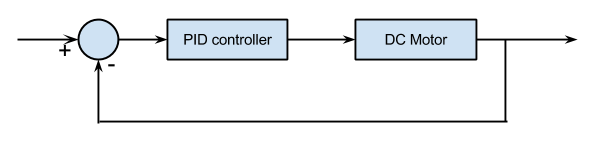
\includegraphics[width=0.5\textwidth]{pid_block_diagram}
	\caption{Block Diagram of the internal closed loop PID Controller}
	\label{fig:pid_block_diagram}
\end{figure}

\begin{figure}[!hbp]
	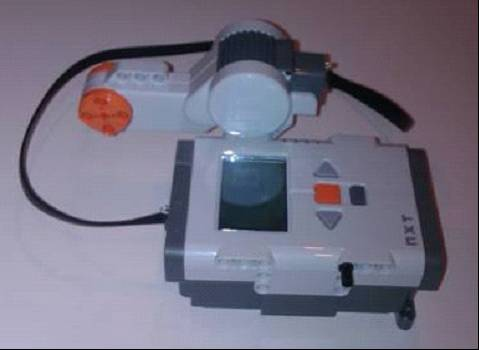
\includegraphics[width=0.5\textwidth]{pid_setup}
	\caption{Experimental setup for observing internal PID Controller}
	\label{fig:pid_setup}
\end{figure}

The LEGO motors are assigned a power rating between $-100$ and $100$ with a negative value denoting reverse direction. Under ideal conditions, the maximum speed of the LEGO motors is $1000$ degrees per second. But this value drops with decrease in battery voltage and increase in motor load. 

The commands for enabling the internal PID Speed Controller and set the maximum regulated speed is:
\begin{verbatim}
nMotorPIDSpeedCtrl[motorB] = mtrSpeedReg;
nMaxRegulatedSpeedNxt = 750;
\end{verbatim}
The internal PID controller provides consistent speed by continuously adjusting the raw power sent to the motor.

The LEGO Intelligent Brick has a \emph{Datalog} feature which allows values to be stored in memory as \verb|(Key,Value)| pairs, which can later be exported to a PC for post-processing. In this experiment, the encoder counts and Motor PWM level are logged every $\Delta{}t  \text{ms}$. The ROBOTC code for this experiment is given below as the motive of this experiment is to get the students acquainted with the software and hardware interfaces. 
\begin{verbatim}
task main()
{
  nMaxRegulatedSpeedNxt = 500;
  // Reset the Motor Encoder
  nMotorEncoder[motorB] = 0;
  nMotorPIDSpeedCtrl[motorB] = mtrSpeedReg;

  int motorRAWpower, motorDegrees;
  motor[motorB] = 50;    // 50/100
  time1[T1] = 0;         // Timer

  // Allocate memory for datalog
  nDatalogSize = 1600;

  while (time1[T1] < 10000) {
    motorDegrees = nMotorEncoder[motorB];
    motorRAWpower = motorPWMLevel[motorB];     
    // store value to Datalog
    AddToDatalog(1,motorPIDdegrees);
    AddToDatalog(2,motorPIDpower);
    wait1Msec(50);
  }
  motor[motorB] = 0;   // Stop the motors
  SaveNxtDatalog();
}
\end{verbatim}

In order to observe the PID control action, the students are asked to run the above program and apply friction on the motor. The internal PID controller will then step in and increase the motor PWM level in order to maintain the speed. This can also be quantitatively verified from the log file. The datalog file (which would be named as \emph{DATAnnnn.rdt}) can be exported to a PC using the \emph{File Management Utility} available in the ROBOTC Development Environment under \emph{Robot$\to$NXT Brick$\to$File Management Utility}. The \emph{Spreadsheet Upload} feature transfers the datalog file to the PC and additionally converts the \emph{.rdt} file into a \emph{.csv} file which can then be processed using any Spreadsheet Processors.

As mentioned earlier, the data is stored as \emph{Key,Value} pairs which constitute the two columns in the exported CSV file. The datalog sequentially stores data with every call to the \verb|AddToDatalog(<index>,<data>);| creating a new entry in the file with a \emph{key} which is proportional to the \emph{index} and the \emph{data} stored as a $16-$bit unsigned integer. Due to this implicit type casting, negative values would get ``wrapped'' around. Hence appropriate post-processing has to be done to handle the same.

The students can now plot the speed in degrees per second and motor PWM level in a single graph to observe the PID action. One such plot is shown in~Figure~\ref{fig:pid_plot}.

\begin{figure}[!hbp]
	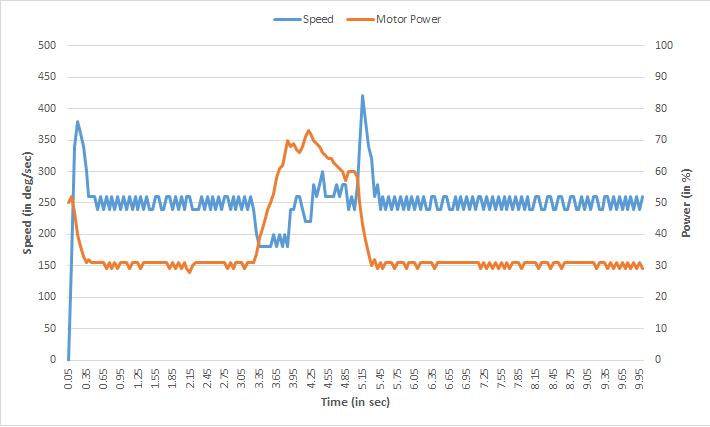
\includegraphics[width=0.5\textwidth]{pid_plot}
	\caption{Plot of Speed vs PWM level of the LEGO motor}
	\label{fig:pid_plot}
\end{figure}

As can be seen from the plot, there is a dip in the speed of the motor between $3$ and $5$ seconds which caused an increase in the PWM power level applied to the motor. When the friction is removed, the speed shoots up due to high power level, before settling down to the desired speed of $250 \deg/s$.

\subsection{Design and tuning of PID controller}
The internal PID controller provided by ROBOTC is sufficient for general purpose use. But in order to understand the characteristics of the DC motor system, writing a custom PID controller would be insightful. In order to implement a custom PID controller, the internal PID controller has to be disabled. The command for disabling the internal PID controller is:
\begin{verbatim}
 nMotorPIDSpeedCtrl[motorB] = mtrNoReg
\end{verbatim}
Once the internal speed regulation is disabled, you can  write your own controller to regulate the speed in order to satisfy desired system characteristics. In this section, you will write a position controller which will regulate the speed so that the motor turns and stops at the desired \emph{setpoint}. The pseudo-code for writing your own PID controller in ROBOTC is given below:
\begin{verbatim}
setpoint = distance in degrees
while(true){
	new err = setpoint-new reading
	diff err = new err-old err
	calculate proportional, integral and derivative constants
	correction = proportional constant + integral constant + derivative constant
	motor PWM = correction
	old err = new err
	store pwm level and current reading to datalog
	wait for few ms
}
\end{verbatim}
Students can follow the provided pseudo-code to design and test custom PID controllers. As shown in the previous experiment, the datalog feature can be used to log data during the experiment and spreadsheet processors can be used to measure the system response. In order to achieve desired system characteristics, the PID parameters need to be tuned. Since we don't have a complete mathematical model of the system, the PID constants cannot be determined through analytic methods. But since we know that DC servo motor is a 3rd order system, we can use Zeigler-Nichols method for calculating the initial value of PID parameters.

\begin{figure}[!hbp]
	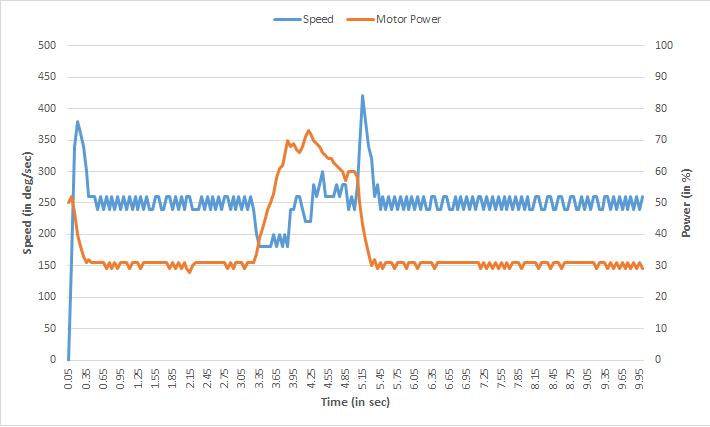
\includegraphics[width=0.5\textwidth]{ZNTuning}
	\caption{Zeigler-Nichols tuning for achieving desired system performance.}
	\label{fig:ZNTuning}
\end{figure}

Students need to understand that a practical DC motor system needs a minimum voltage in order to start rotating. Also, the difference in static and dynamic friction coefficients will have an effect in the minimum voltage required. While employing Zeigler-Nichols tuning, the setpoint must be chosen to be large enough to produce a significant voltage output. Also, the calculated PWM level must be constrained to the range $[-100,100]$ to avoid unexpected behaviours due to ``wrapping''.

For more details on Zeigler-Nichols method, refer~\cite{Appendix:ZN}. The initial PID parameters obtained using Z-N method may not satisfy the design characteristics. Therefore, the PID parameters are tuned through ``informed trial and error'' to achieve the desired system performance. See~Figure~\cite{fig:ZNTuning} for an example.

\subsection{System Identification using MATLAB}
System Identification is the process of deriving a mathematical model of the system under consideration using experimental data. In the previous experiment, we adopted ``trial and error'' methods for calculating the parameters for implementing a closed-loop PID controller. In this experiment, we will focus on deriving a complete mathematical model of the DC motor system so that analytical methods can be employed for calculating the PID parameters and verified on the real-world system.

MATLAB provides System Identification toolbox which can be used to estimate transfer function models of an experimental system using the input/ouput data. System Identification is in itself a vast field and hence we will explain only the features required for this experiment. In brief, system identification involves a 3-step loop - 1. Data acquisition, 2. Estimate Mathematical model and 3. Verify the derived model. For this and the next part of this section, MATLAB and Simulink will be the used as the programming environment. This requires updating the LEGO kit firmware with the ``enhanced standard firmware''. Refer~Appendix\cite{Appendix:Firmware} for detailed instructions.

\subsubsection{Data Acquisition}
The first step in system identification is acquiring ``\emph{good data}''. This is done by exciting the system using a well-designed input signal and measuring the system response. A well-designed input signal should excite the system with all frequencies. The estimated mathematical model can only be as accurate as the acquired data. But there are fundamental constraints in measuring data which are introduced by the quantizations in the optical position encoder of the motor, time delay in motor response, discrete time data acquisition etc\ldots For the lego DC motor system, the dominant constraint is the low resolution of the rotary encoder which has a least count of $1\deg$.

\begin{figure}[!hbp]
	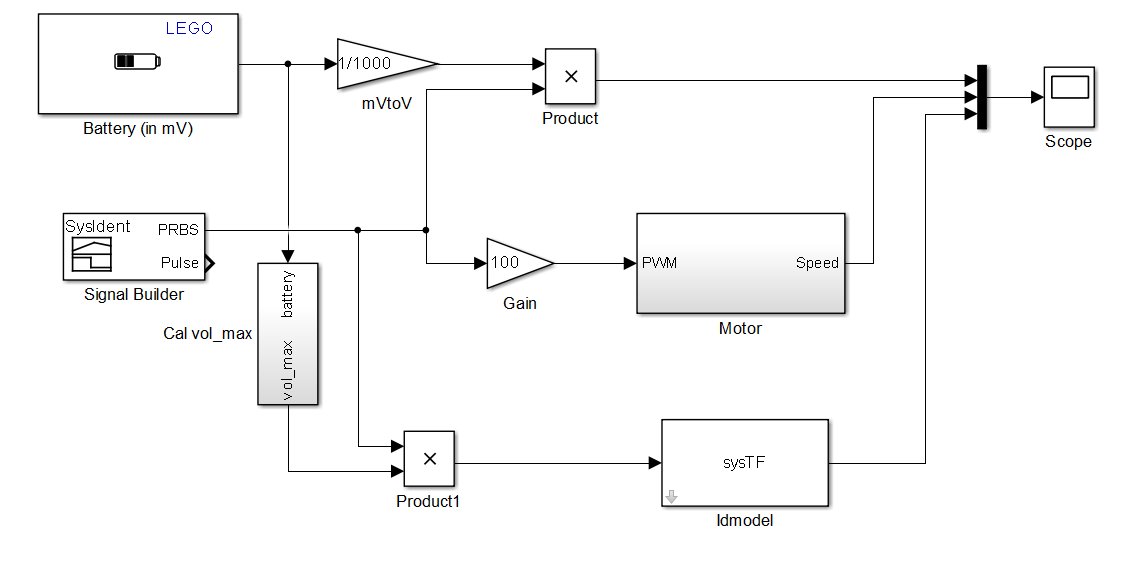
\includegraphics[width=0.5\textwidth]{tf_daq_model}
	\caption{Simulink block diagram for data acquisition}
	\label{fig:tf_daq_model}
\end{figure}

In order to obtain``\emph{good data}'', the system needs to excited using a wide bandwidth signal around the natural operating frequency. This can  be achieved by using the \verb|Signal Builder| block in Simulink. A \emph{Pseudorandom noise} signal with a frequency of $0.5Hz$ is used to control the LEGO motor. The output of the system is obtained using the \verb|Encoder| block which provides the total degrees rotated by the motor. This time domain input-output data is exported into workspace by using the \verb|scope| block. Refer~Figure\cite{fig:tf_daq_model} for the complete Simulink block diagram. While the input to the \verb|Motor| block in Simulink toolbox is PWM duty ratio, the actual input to the system is \verb|voltage|. Due to various non-idealities, the PWM to voltage mapping is not linear, especially as the battery voltage does not remain constant throughout the operation. Hence, emperical results are used to calculate the maximum voltage supplied to the lego motors for a given battery voltage.\cite{ref:Yamamoto}. This Simulink model is then run in \emph{external} mode in order to let the \verb|scope| log the data from the \verb|Intelligent Brick| in real-time. Due to various reasons, the data-logging begins only after a few hundred milliseconds and hence the input is given after $1 sec$. 

\subsubsection{Estimate Mathematical Model}
The next step in system identification is to fit a mathematical model to the acquired data. This process is simplified by using System Identification Toolbox in MATLAB. In this experiment, we will estimate the transfer function model of the DC motor system using the measured signal data. The code snippet for achieving this is given below. For more details on transfer function estimation, refer MATLAB's tutorial on \emph{Estimating Transfer Function Models for a Heat Exchanger}.
\begin{verbatim}
% Assuming scope data is stored in motorResponse variable.
u1 = motorResponse(:,2); % Voltage
y1 = motorResponse(:,3); % Speed
data = iddata(y1,u1,Ts);
sysTF = tfest(data,2,0);
\end{verbatim}
\begin{figure}[!hbp]
	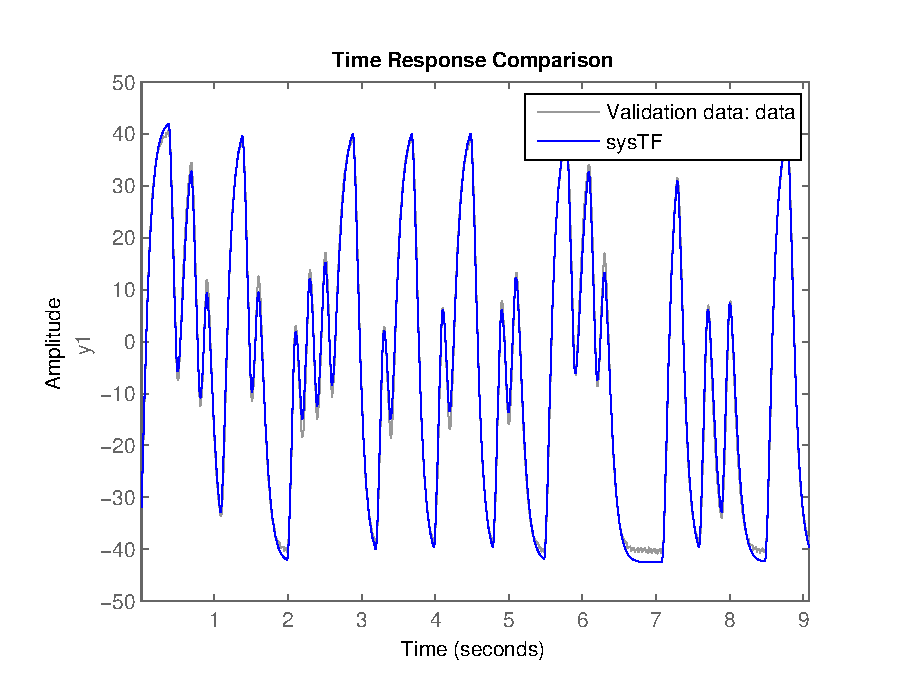
\includegraphics[width=0.5\textwidth]{tf_validate}
	\caption{Estimated transfer function model}
	\label{fig:tf_validate}
\end{figure}
The quality of fit can be analysed using \verb|compare| and \verb|residue| commands as shown in~Figure~\cite{fig:tf_validate}. It is recommended to have 70\%-30\% split of the acquired data. The larger portion is used to estimate the transfer function while the smaller portion is used to validate the model. This helps in detecting \emph{over-fitting}.

\subsubsection{Verification}
The final step in system identification is to verify the model in real-time. This can be achieved by simultaneously exciting the system and the transfer function model with a pulse input and comparing the outputs. The \verb|idmodel| block can be used in Simulink to import the transfer function model from the workspace. The complete block diagram for the verification is shown in~Figure~\cite{fig:tf_verify}.

\begin{figure}[!hbp]
	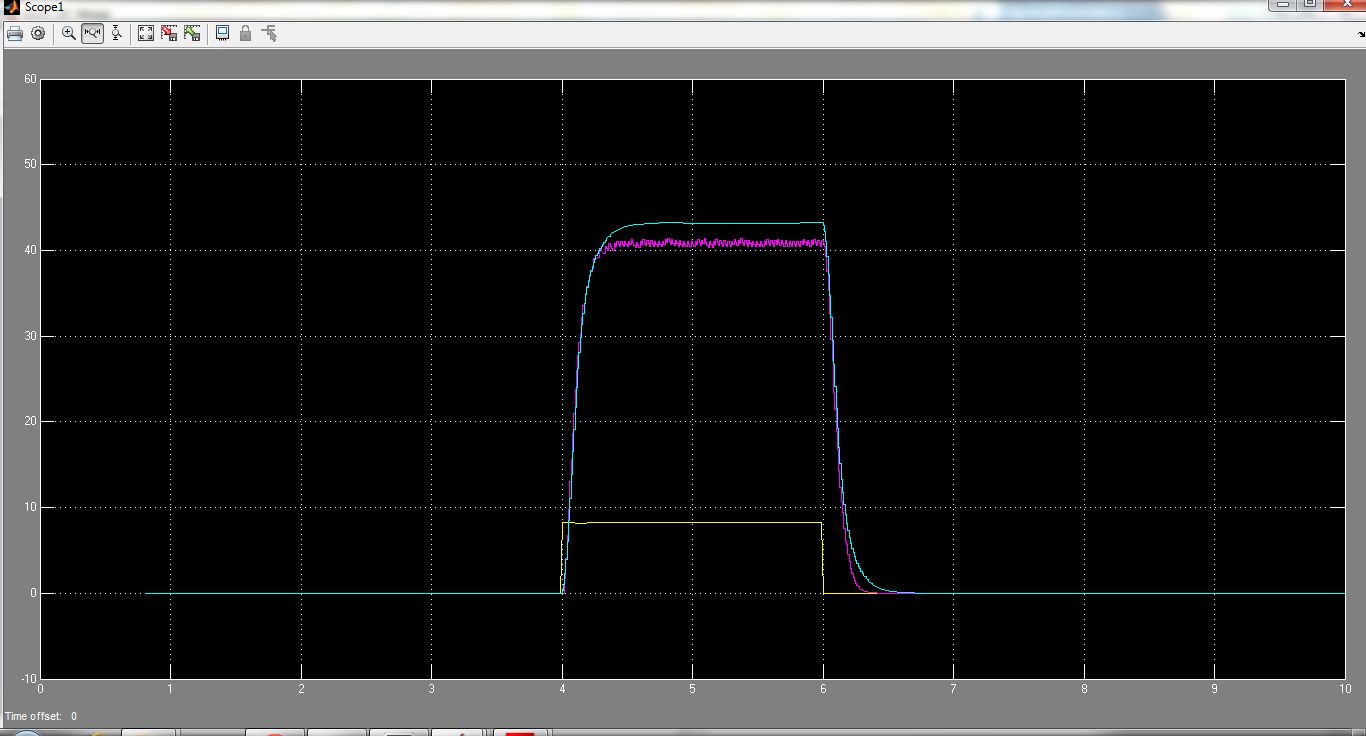
\includegraphics[width=0.5\textwidth]{tf_verify}
	\caption{Simulink block diagram for verifying the estimated mathematical model.}
	\label{fig:tf_verify}
\end{figure}

\subsection{Proportional controller design using Root-Locus}
In the previous experiment, we derived the complete mathematical model of the DC motor system. In this experiment we will use this model to design a closed loop Proportional controller for critically damped system response. The Control System toolbox in MATLAB provides many useful functions for performing \emph{Root-Locus} analysis. The proportional gain for the controller can be determined from the open loop transfer function as follows:
\begin{verbatim}
sys=tf([212.4],[1 172.3 2826]);
[Kp,poles]=rlocfind(sys,[-86.15]);
\end{verbatim}
The calculated $Kp$ value is used in the closed loop proportional controller for the DC motor system. The overall closed-loop transfer function has a DC gain of $H(0)=0.6192$. Therefore, a compensating gain of $1/H(0)$ needs to be added in series as shown in~Figure~\cite{fig:tf_pid}.

\begin{figure}[!hbp]
	\includegraphics[width=0.5\textwidth]{tf_pid}
	\caption{Simulink block diagram for Proportional Controller for DC motor system.}
	\label{fig:tf_pid}
\end{figure}

Students can repeat the process for achieving different system characteristics and verify by implementing in the \emph{Intelligent Brick}.
\section{Conclusions for Analysis of LEGO DC Motor}
Concepts learned: Block Diagram, Feedback control, Open loop and closed loop control, PID controller, Zeigler-Nichols tuning, transfer function, system identification and verification, bode plots, Root-Locus analysis etc...

\section{Mobile Inverted Pendulum using LEGO Mindstorms}
This section details the building of a Mobile Inverted Pendulum(MIP) robot using the LEGO Mindstorms kit and a HiTechnic Gyro Sensor. The MIP system is a well studied classic problem in Control Engineering. This makes it ideal for a 1 month course project in a first year Masters programme in Control Engineering. There are plenty of online resources for building the MIP robot which is popularly referred as \emph{NXTway-GS}. An exhaustive documentation for this project is given in the paper \emph{NXTway-GS A Model Based Design} by Yamamoto.\cite{ref:Yamamoto}. The Simulink model for NXTway-GS is also provided as an example along with the NXT Hardware Support package. This model will be used as the starting point for our analysis of this MIP robot. 

\subsection{Modifying the MIP robot}


\subsection{Controller Design}
Linearization about $\psi = 0$
State space representation 
Servo controller
Feedback gain calculations - LQR concepts
Integral gain to regulate steady state errors.

\subsection{Simulation and Verfication}
Simulation results
experimental results
graphs and diagrams

\section{Conclusions for Mobile Inverted Pendulum robot}
Summary of concepts learned through this project.
Time frame for the project.
Possible alterations

\section{Pendulum on a Cart system}
This section details the building of a Pendulum on a Cart system. The objective of this experiment is to design a feedback-based controller in order to minimize the swinging of the pendulum while moving in a straight line path. The feedback is provided by an NXT Angle Sensor from HiTechnic which has a least-count of $1\deg$. The controller must damp any external disturbances as well as the swinging caused due to the linear acceleration of the cart. A valuable reference for this project is the paper \emph{Using LEGO in Control Education} by Peter~J.~Gawthrop and Euan~McGookin\cite{ref:gawthrop}. MATLAB/Simulink will be used as software for this project as well. 

\subsection{Building the Cart and Pendulum system}

\subsubsection{Adjusting weight balance}

\subsubsection{Calibrating the Angle Sensor}

\subsection{System Identification}

\subsection{Controller Design}

\subsubsection{Velocity control}

\subsubsection{Load position control}

\subsubsection{Cart position control}

\subsection{Future work}

\section{Conclusions for Pendulum on a Cart system}

\section{Appendix}
\subsection{Zeigler-Nichols Tuning}
\begin{itemize}
\item Set Ki and Kd to zero.
\item Slowly increase Kp to a value Ku at which sustained oscillations - constant amplitude and periodic - are observed.
\item Note period of oscillation
\item Refer table below for initial values
\end{itemize}

\begin{tabular}{|l|l|l|l|}
\hline
       Z-N Model      & Kp       & Ki       & Kd       \\      
\hline
       P controller   & 0.5*Ku   & 0        & 0        \\
\hline
       PI controller  & 0.455*Ku & 0.833*Tu & 0        \\
\hline
       PID controller & 0.588*Ku & 0.5*Tu   & 0.125*Tu \\
\hline
\end{tabular}
\\
\\
Since Z-N method usually results in aggressive tuning, alternatively Tyreus-Luyben method can be adopted.
\\
\begin{tabular}{|l|l|l|l|}
\hline
       T-L Model      & Kp       & Ki     & Kd       \\
\hline
       PI controller  & 0.312*Ku & 2.2*Tu & 0        \\
\hline
       PID controller & 0.454*Ku & 2.2*Tu & 0.159*Tu \\
\hline
\end{tabular}

\subsection{Programming LEGO NXT kits using Simulink}
MATLAB and Simulink provides many \emph{hardware support} packages for developing standalone algorithms which can be directly deployed in the target hardware of choice from Simulink. A wide variety of platforms are supported which include Arduino, Raspberry Pi and LEGO Mindstorms NXT and EV3 as well. The \emph{Hardware Support} packages can be installed using \verb|supportPackageInstaller| command in MATLAB command window.
Alternatively, the LEGO NXT kit can be controlled from MATLAB using RWTHMindstormsNXT toolbox. This MATLAB toolbox largely developed by members of RWTH Aachen University, provides matlab scripts for communication with the LEGO NXT Intelligent brick and to interface with the motors and sensors that are attached to the Intelligent brick.

\subsection{Updating firmware of LEGO Intelligent Brick}

%%% End document
\end{document}